%%%%%%%%%%%%%%%%%%%%%%%%%%%%%%%%%%%%%%%%%%%%%%%%%%%
%
%  New template code for TAMU Theses and Dissertations starting Fall 2016.  
%
%
%  Author: Sean Zachary Roberson
%  Version 3.17.09
%  Last Updated: 9/21/2017
%
%%%%%%%%%%%%%%%%%%%%%%%%%%%%%%%%%%%%%%%%%%%%%%%%%%%
%%%%%%%%%%%%%%%%%%%%%%%%%%%%%%%%%%%%%%%%%%%%%%%%%%%%%%%%%%%%%%%%%%%%%%
%%                           SECTION III
%%%%%%%%%%%%%%%%%%%%%%%%%%%%%%%%%%%%%%%%%%%%%%%%%%%%%%%%%%%%%%%%%%%%%

\chapter{RESULTS}
The radio altimeter tests described in this work were developed over a two year long process which can be approximately separated into three distinct phases of testing. The initial testing results discussed in Section~\ref{sec:initial_results} characterized the basic response of altimeters to various types of interference. These led to another set of tests aimed at more systematically demonstrating altimeter performance under more conservative than real life conditions. The in band testing in Section~\ref{sec:dvsg_ib_results} demonstrated what power level of a full 200MHz of WAIC interferers would break an altimeter in the worst case scenario. Finally, the Out of Band testing regimen investigated altimeter performance when subjected to cellular interference in neighboring bands. Preliminary out of band results are discussed in Section~\ref{sec:dvsg_oob_results}. Results of the two later testing regimens were used to propose maximum radiated power values to  regulators, as well as in continuing discussions. 

\section{General Plotting Scripts}
This setup shows introduces the two general types of plots used across all tests, called `Height Plots' and `Stat Plots' respectively. The form of these was evolved over the course of different testing regimens to communicate the results from each effectively, but the basic plots introduce a standard format in which results from an altimeter test are displayed. 
\subsection{Height Plots}
The first attempts at a representation of data taken during these tests developed into \textit{height plots}. The goal of the height plot is to provide a visualization of how the interference signals from the VSG  distort the altitude signal output by an altimeter over time. In each altimeter test, a height plot is generated for each unique combination of center frequency and modulation format under test. Figure~\ref{fig:height_plot_example} shows an height plot from the initial testing regimen. 

\begin{figure}[h!]
	\centering
	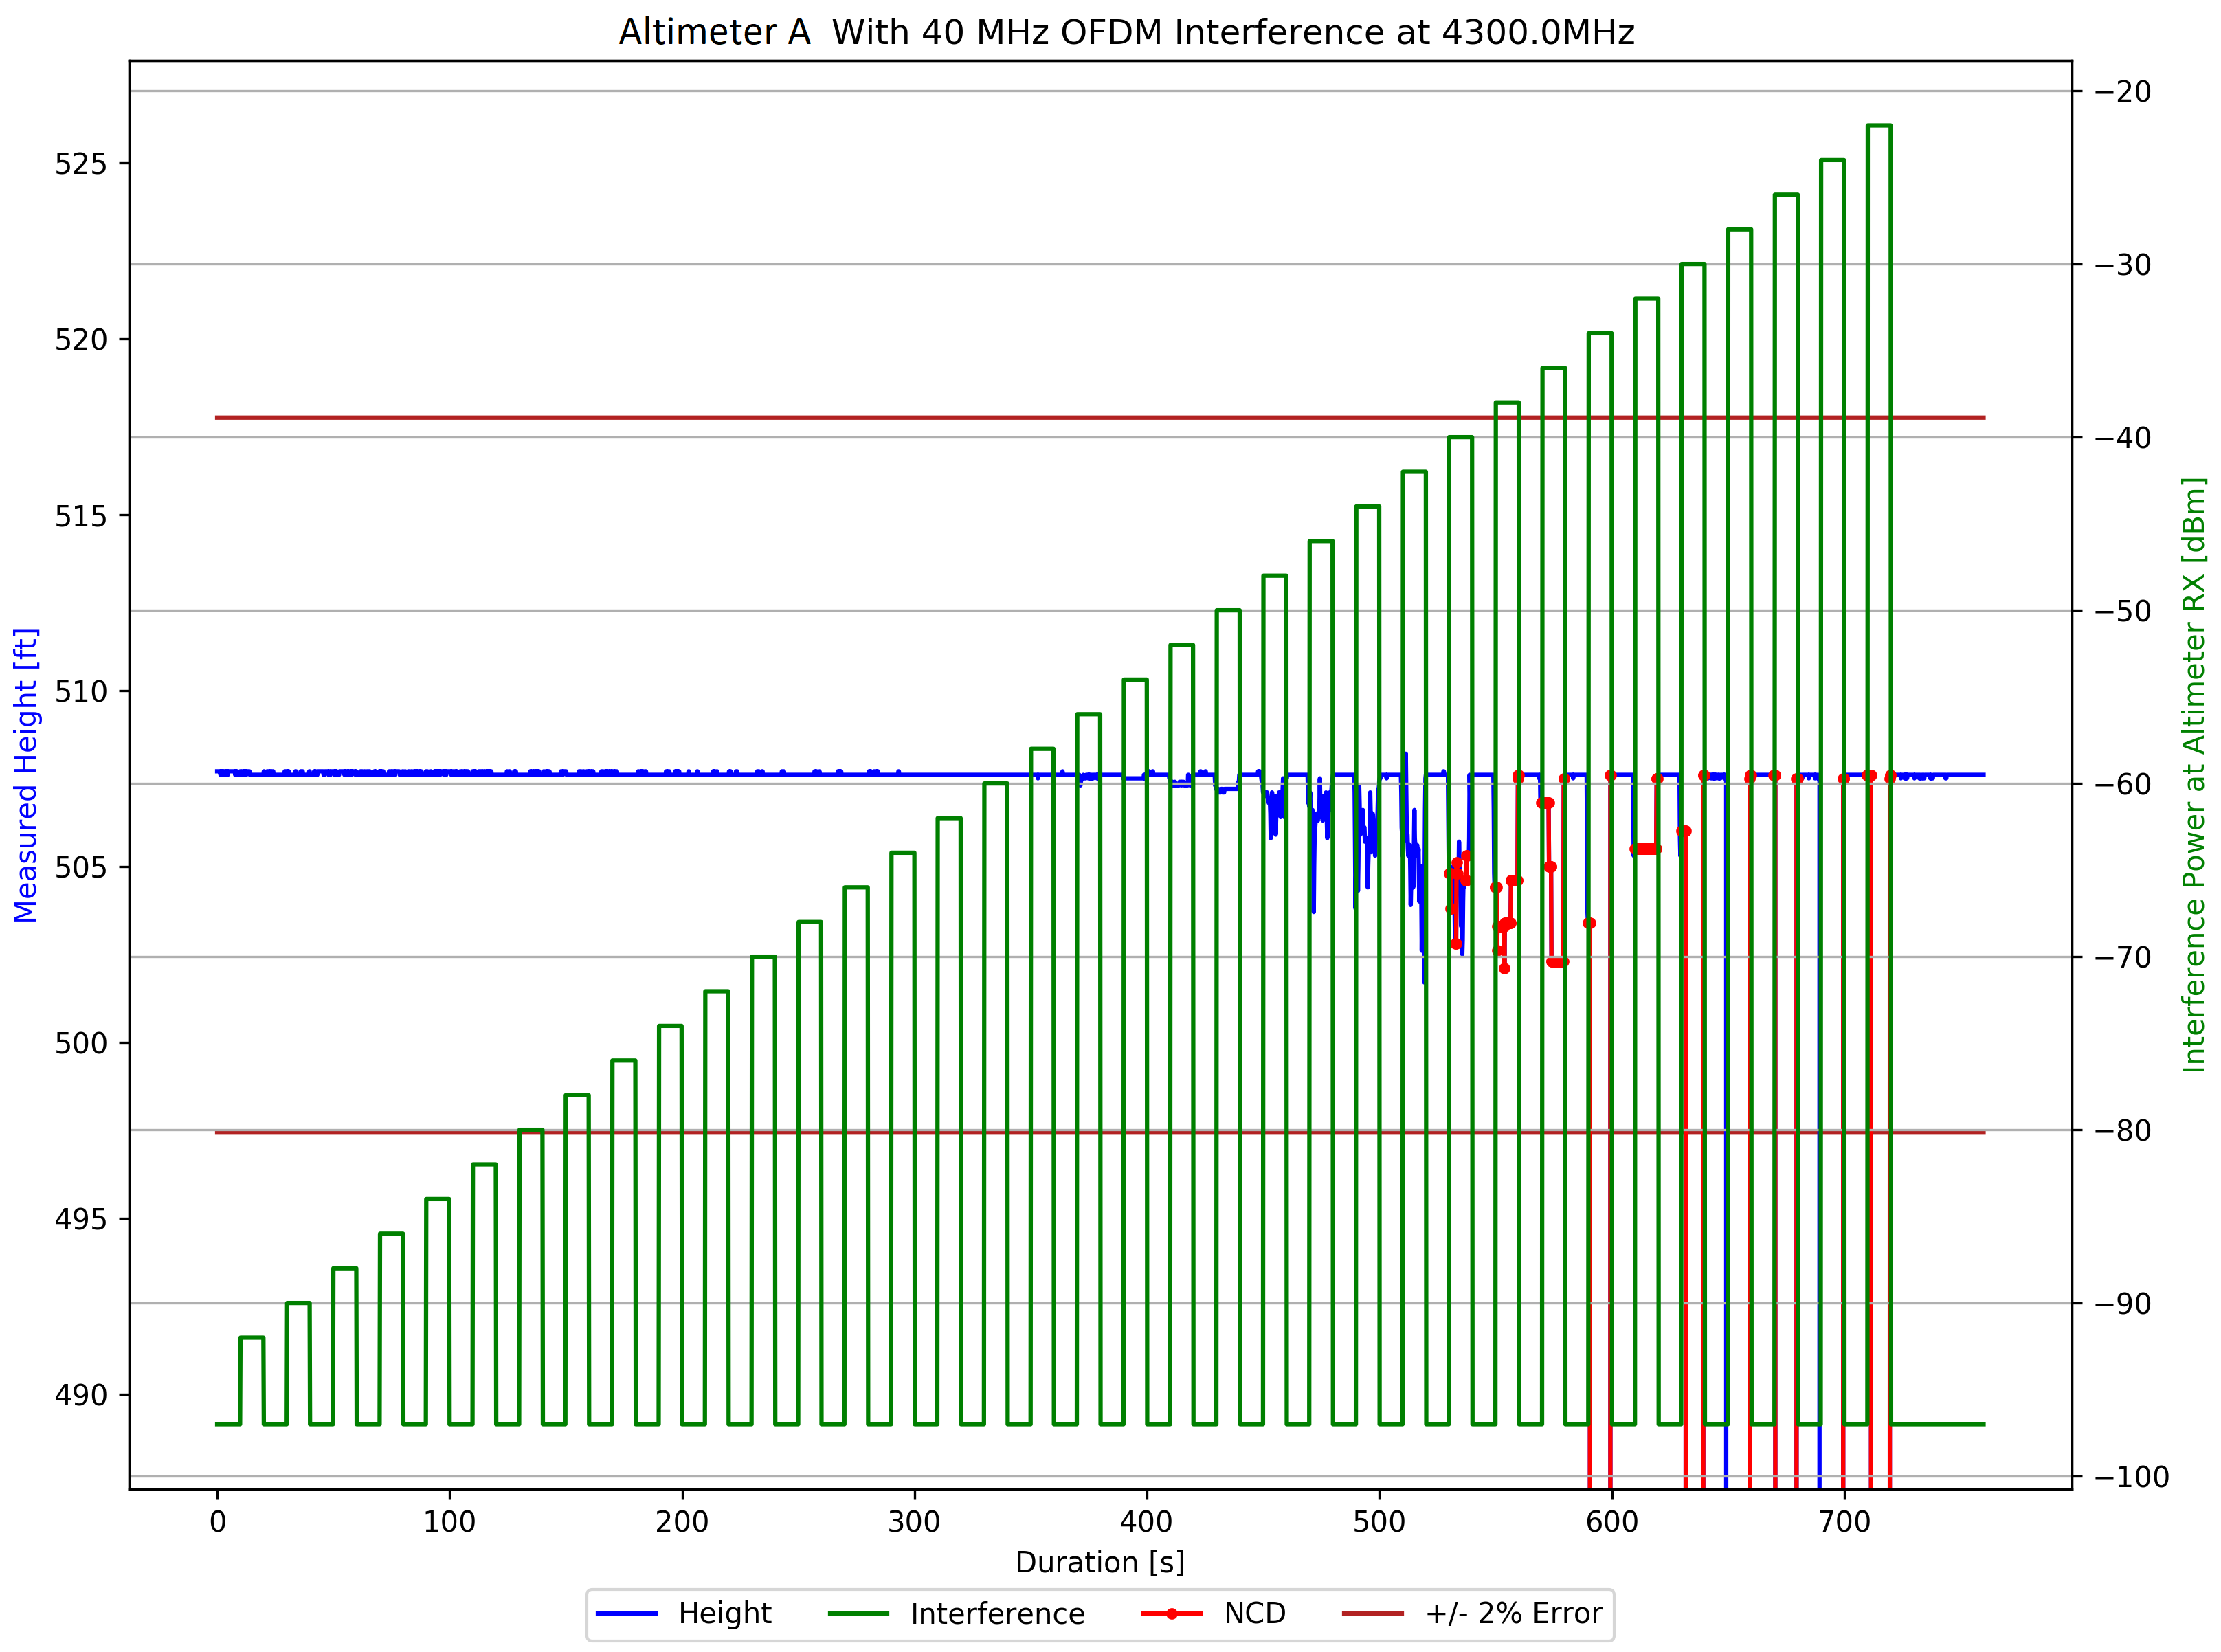
\includegraphics[width=6.0in]{Example_Height_Plot.png}
	\caption{Example Height Plot from Initial Testing Regimen}
	\label{fig:height_plot_example}
\end{figure}
Important information about the test being displayed is contained in the title of each height plot. This includes the altimeter make and model, the bandwidth and modulation format of the interference signal being tested, and the center frequency of RF carrier setting used by the VSG.

The x-axis shows the test duration in seconds. After the SQL query sorts by modulation and carrier, the zero second point is set to correspond to the start time for the first RF OFF state for the first interference signal. This time-stamp is subtracted from every mapped data point to yield a plot vs test duration in seconds.

The left hand y-axis shows the height output by an altimeter in feet. The axis is centered about \textit{correct height} calculated as the median height before any interference is turned on (See Section~\ref{subsub:nominal}). The upper and lower bounds of this axis correspond to $\pm4$\% error from this correct height respectively. The height signal is plotted with a blue line, but for measurements labeled NCD by the device under test, this is replaced with a bright red marker to clearly show the failure state. Finally, the burgundy lines show the ARINC 707 specified $\pm2$\% error margins. Measurements passing this value constitute a device no longer meeting specifications for certification and are considered severe.  

Finally, the right hand y-axis corresponds to the interference power level experienced by the altimeter receiver. The green staircase waveform shows how the RF generator was toggled on and off in increasing power levels over time. To easily signal an OFF state, the OFF state was plotted on the same line as the ON state, with 5 dB subtracted from the minimum interference power used in a test. 

Displaying the data in height plots has numerous advantages. This format clearly shows how an altitude signal is distorted with increasing interference power over time, as well as how quickly the altimeter recovers once the interference is turned off. This format also allows the point in time an altimeter outputs NCD to easily be located. The plots versus time were extremely useful in debugging a test. Errors such as an altimeter which stops outputting data in the middle of a test manifest themselves clearly in a height plot, and manufacturers can correlate this data with recordings of the internal signal processing data stored on SD cards during a test.  
\subsection{Stat Plots}
Despite the advantages stated above, height plots had a disadvantage of being extremely cluttered. When presenting test results to regulators, members of the project management committee tended to spend a disproportionate amount of time discussing the different aspects of the data display as opposed to the results themselves. This motivated the development of stat plots.

Figure~\ref{fig:stat_plot_example} shows an example stat plot made from the same data as the Height Plot in Figure~\ref{fig:height_plot_example}. Stat plots show height error from the correct height versus RF power at the altimeter receiver when the RF power is on. The mean, max, and min are all plotted along with standard deviation error bars and a marker to indicate NCD. Because the noise caused by interference power is not necessarily a normal distribution, the standard deviation error bars do not necessarily have the precise meaning they do with Gaussian noise. However, the error bars do provide a visual representation for how much variance from the mean a given RF power causes. Because of this, they are kept in the plot as a good way to communicate the data.  
\begin{figure}[h!]
	\centering
	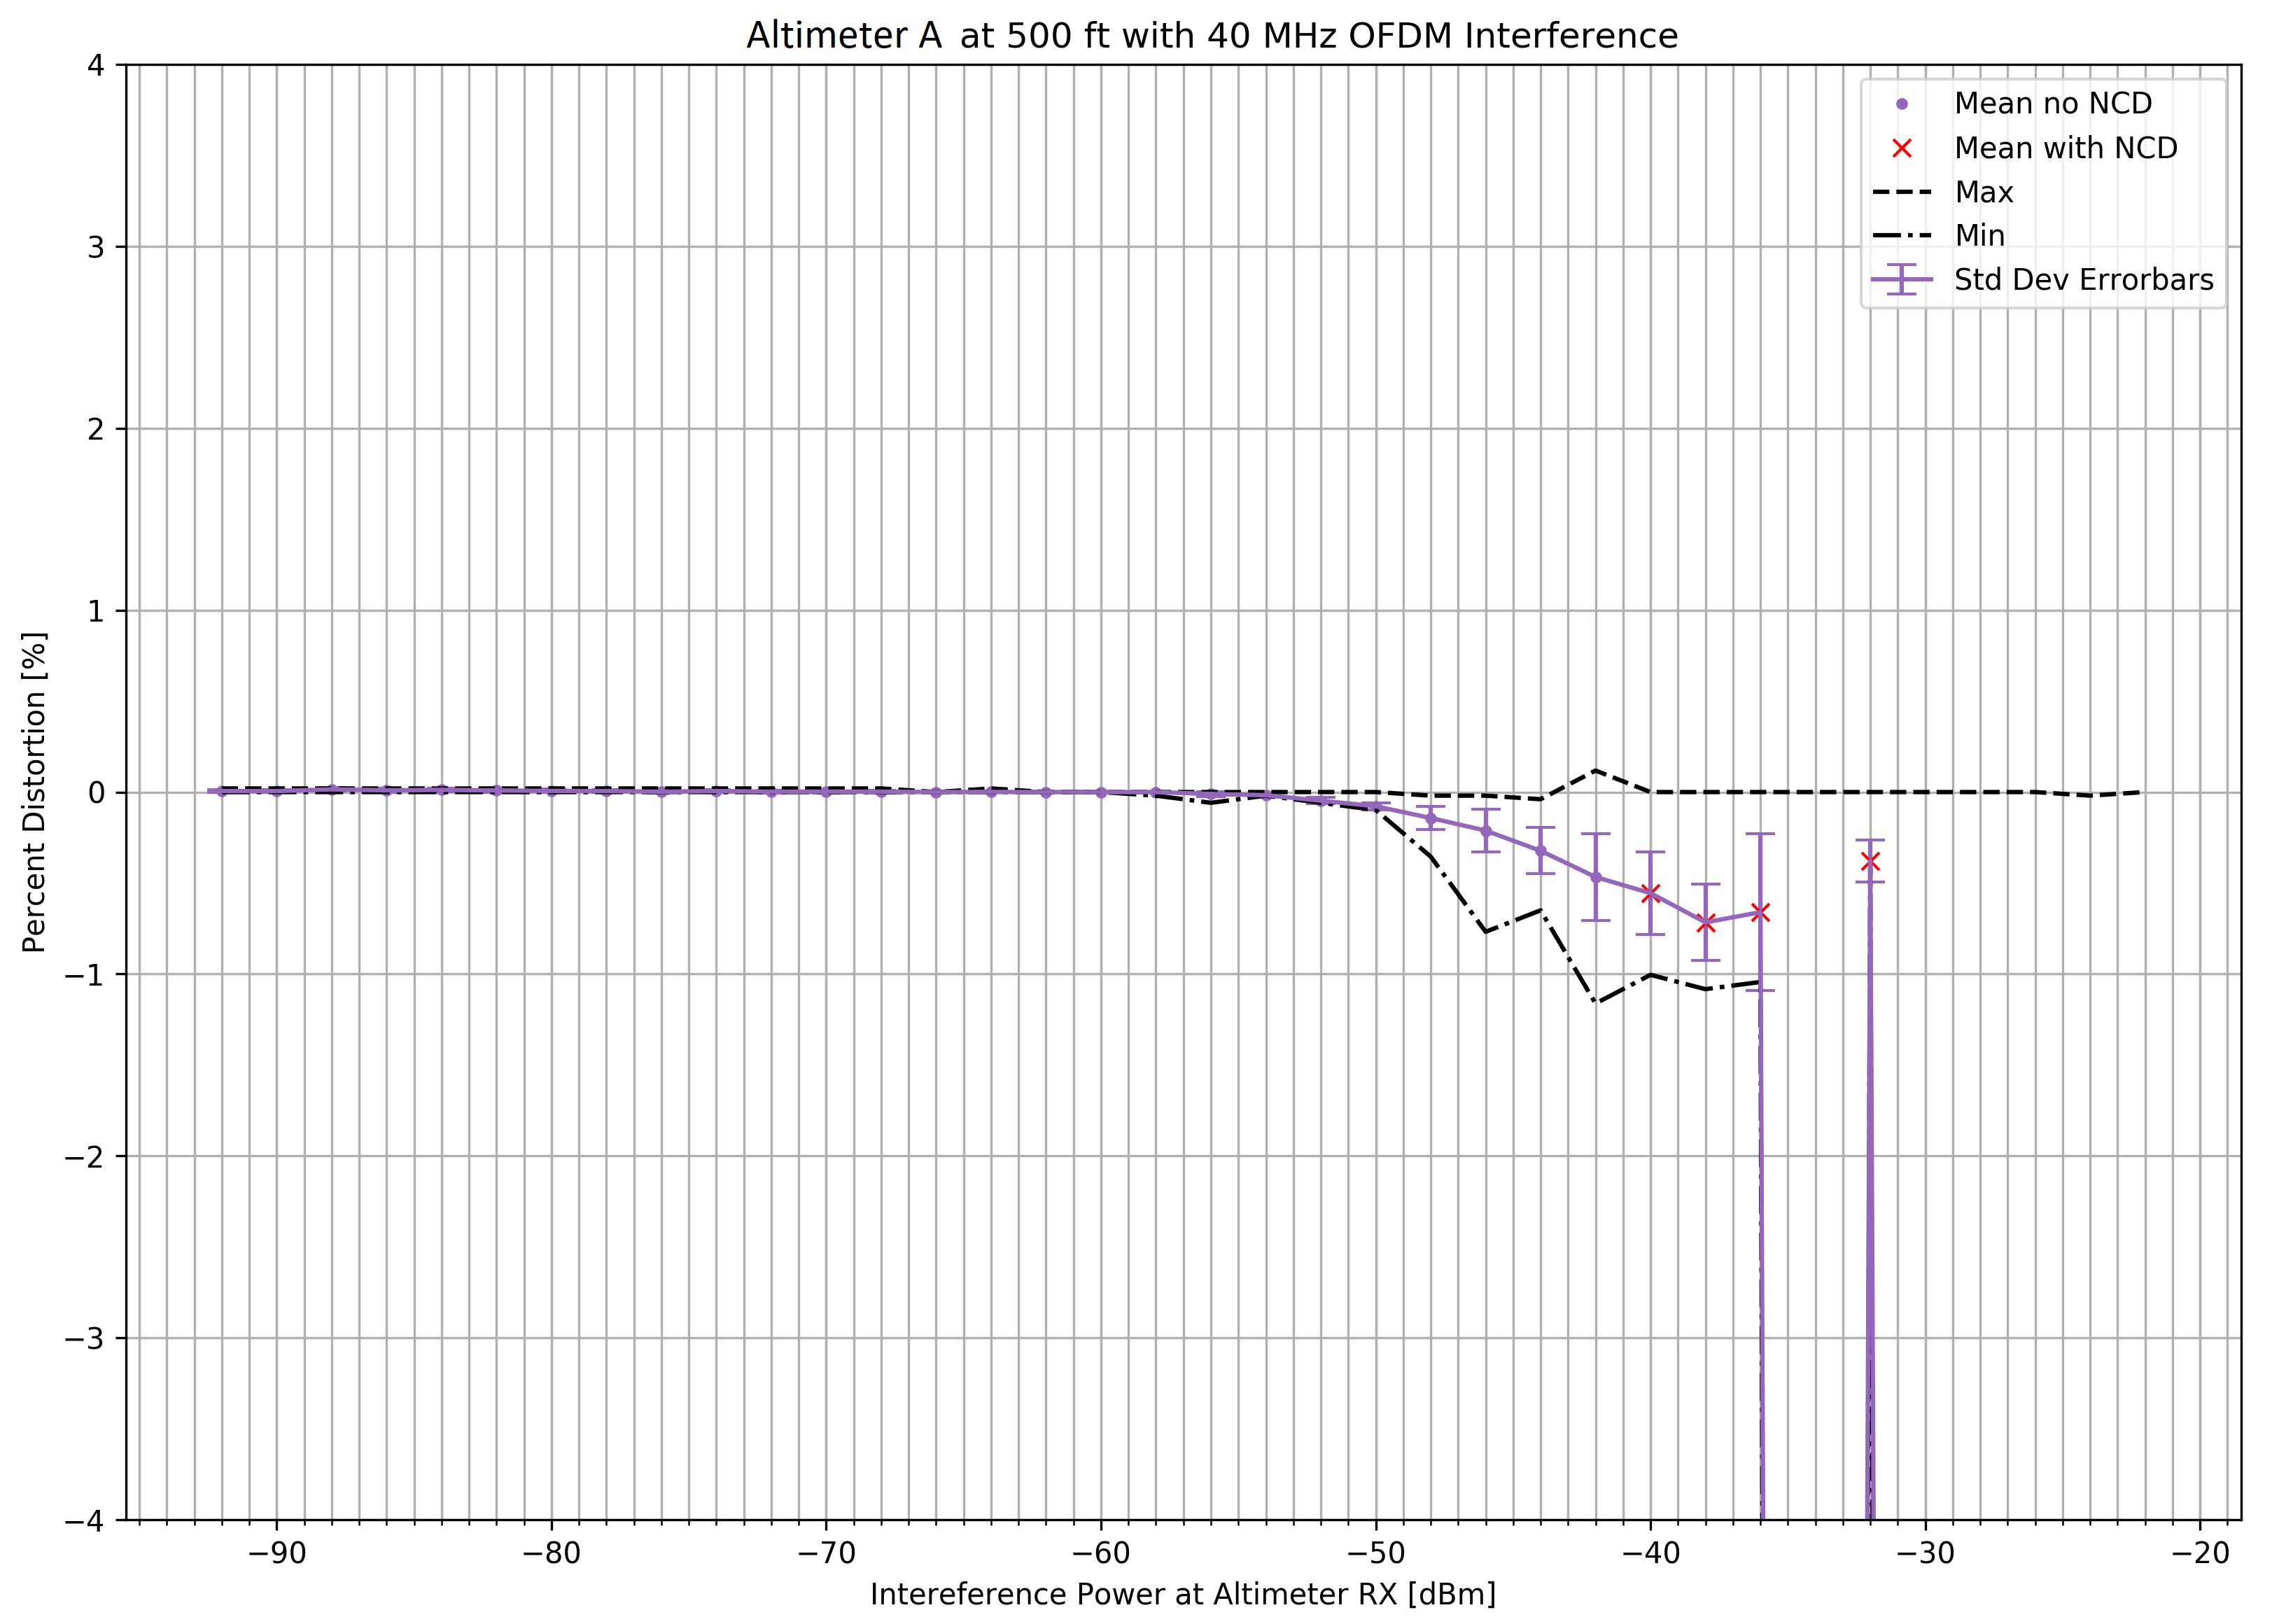
\includegraphics[width=6.0in]{Example_Stat_Plot.png}
	\caption{Example Stat Plot}
	\label{fig:stat_plot_example}
\end{figure}

 Although stat plots do not contain any information about the timing of different events in an altimeter test, they provide a more concise and clean method to display the results of an altimeter test. These features led this representation to be used to communicate test results in letters to the International Civil Aviation Organization (ICAO) Frequency Spectrum Management Panel (FSMP)~\cite{uwe_radio_2019}. 
 
 
\section{Initial `WAIC Only' Testing Regimen}\label{sec:initial_results}
This Section covers the results of the initial testing regimen described in Section~\ref{sec:initial}. The `WAIC only' testing was a long term, multifaceted investigation which characterized various aspects of the altimeter response to interference. The test definition from Table~\ref{tab:initial_signals} shows a representative example of a test run with a single altimeter. This would be repeated for the 5 different commercial altimeters sampled for these tests, and for each height the test setup was capable of. 
\begin{figure}[h!]
	\centering
	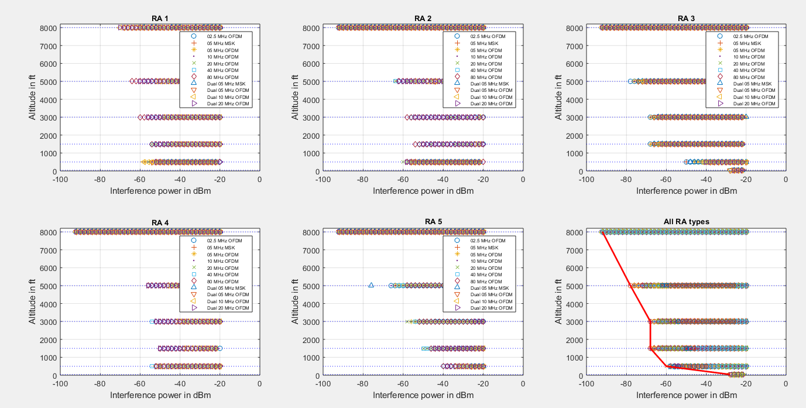
\includegraphics[width=6.0in]{Initial_Summary.png}
	\caption{Summary of Initial Testing Results Presented to the FSMP in~\cite{uwe_radio_2019}}
	\label{fig:initial_summary}
\end{figure}

Figure~\ref{fig:initial_summary} shows a comprehensive summary of these results. Each data point on shows the results of a single altimeter test equivalent to a height plot in Figure~\ref{fig:height_plot_example}. The data points plot the power level at which the altimeter under test goes beyond a mean error of $\pm0.5\%$. This plot served as an introduction to the presentation of the results of the second and third testing regimens~\cite{uwe_radio_2019}, as a means of showing how the WAIC only tests justified further investigation. 

Early tests investigated the proper loop loss value to use. Although loop losses were specified in DO-155 (See Section~\ref{subsub:loss}), it was ambiguous as to whether the loop losses were to be measured between the ports of the altimeter or between the ports of the altitude simulator. While the language in the regulations made it seem intuitive to place the loop loss between the ports of the altitude simulator, the additional cable loss leading to and from the simulator made the altimeters unable to function. It was hypothesized that the worst case scattering coefficients in use for the loop loss calculation made the addition of cabling turn an already conservative case to an unrealistic one. Because these units were all certified, the loop loss was moved to the ports of the altitude simulator to ensure functionality, and this was noted in any communication of results to outside parties.

A series of tests during the initial testing regimen placed a 10 MHz OFDM signal at different points in the altimeter band. These showed that the altimeter under test consistently broke at lower power levels when interference was injected at the center of the band than at the outer edges. Subsequent testing only centered simulated WAIC waveforms at the center of the band to provide the most conservative results. 
\begin{figure}[h!]
	\centering
	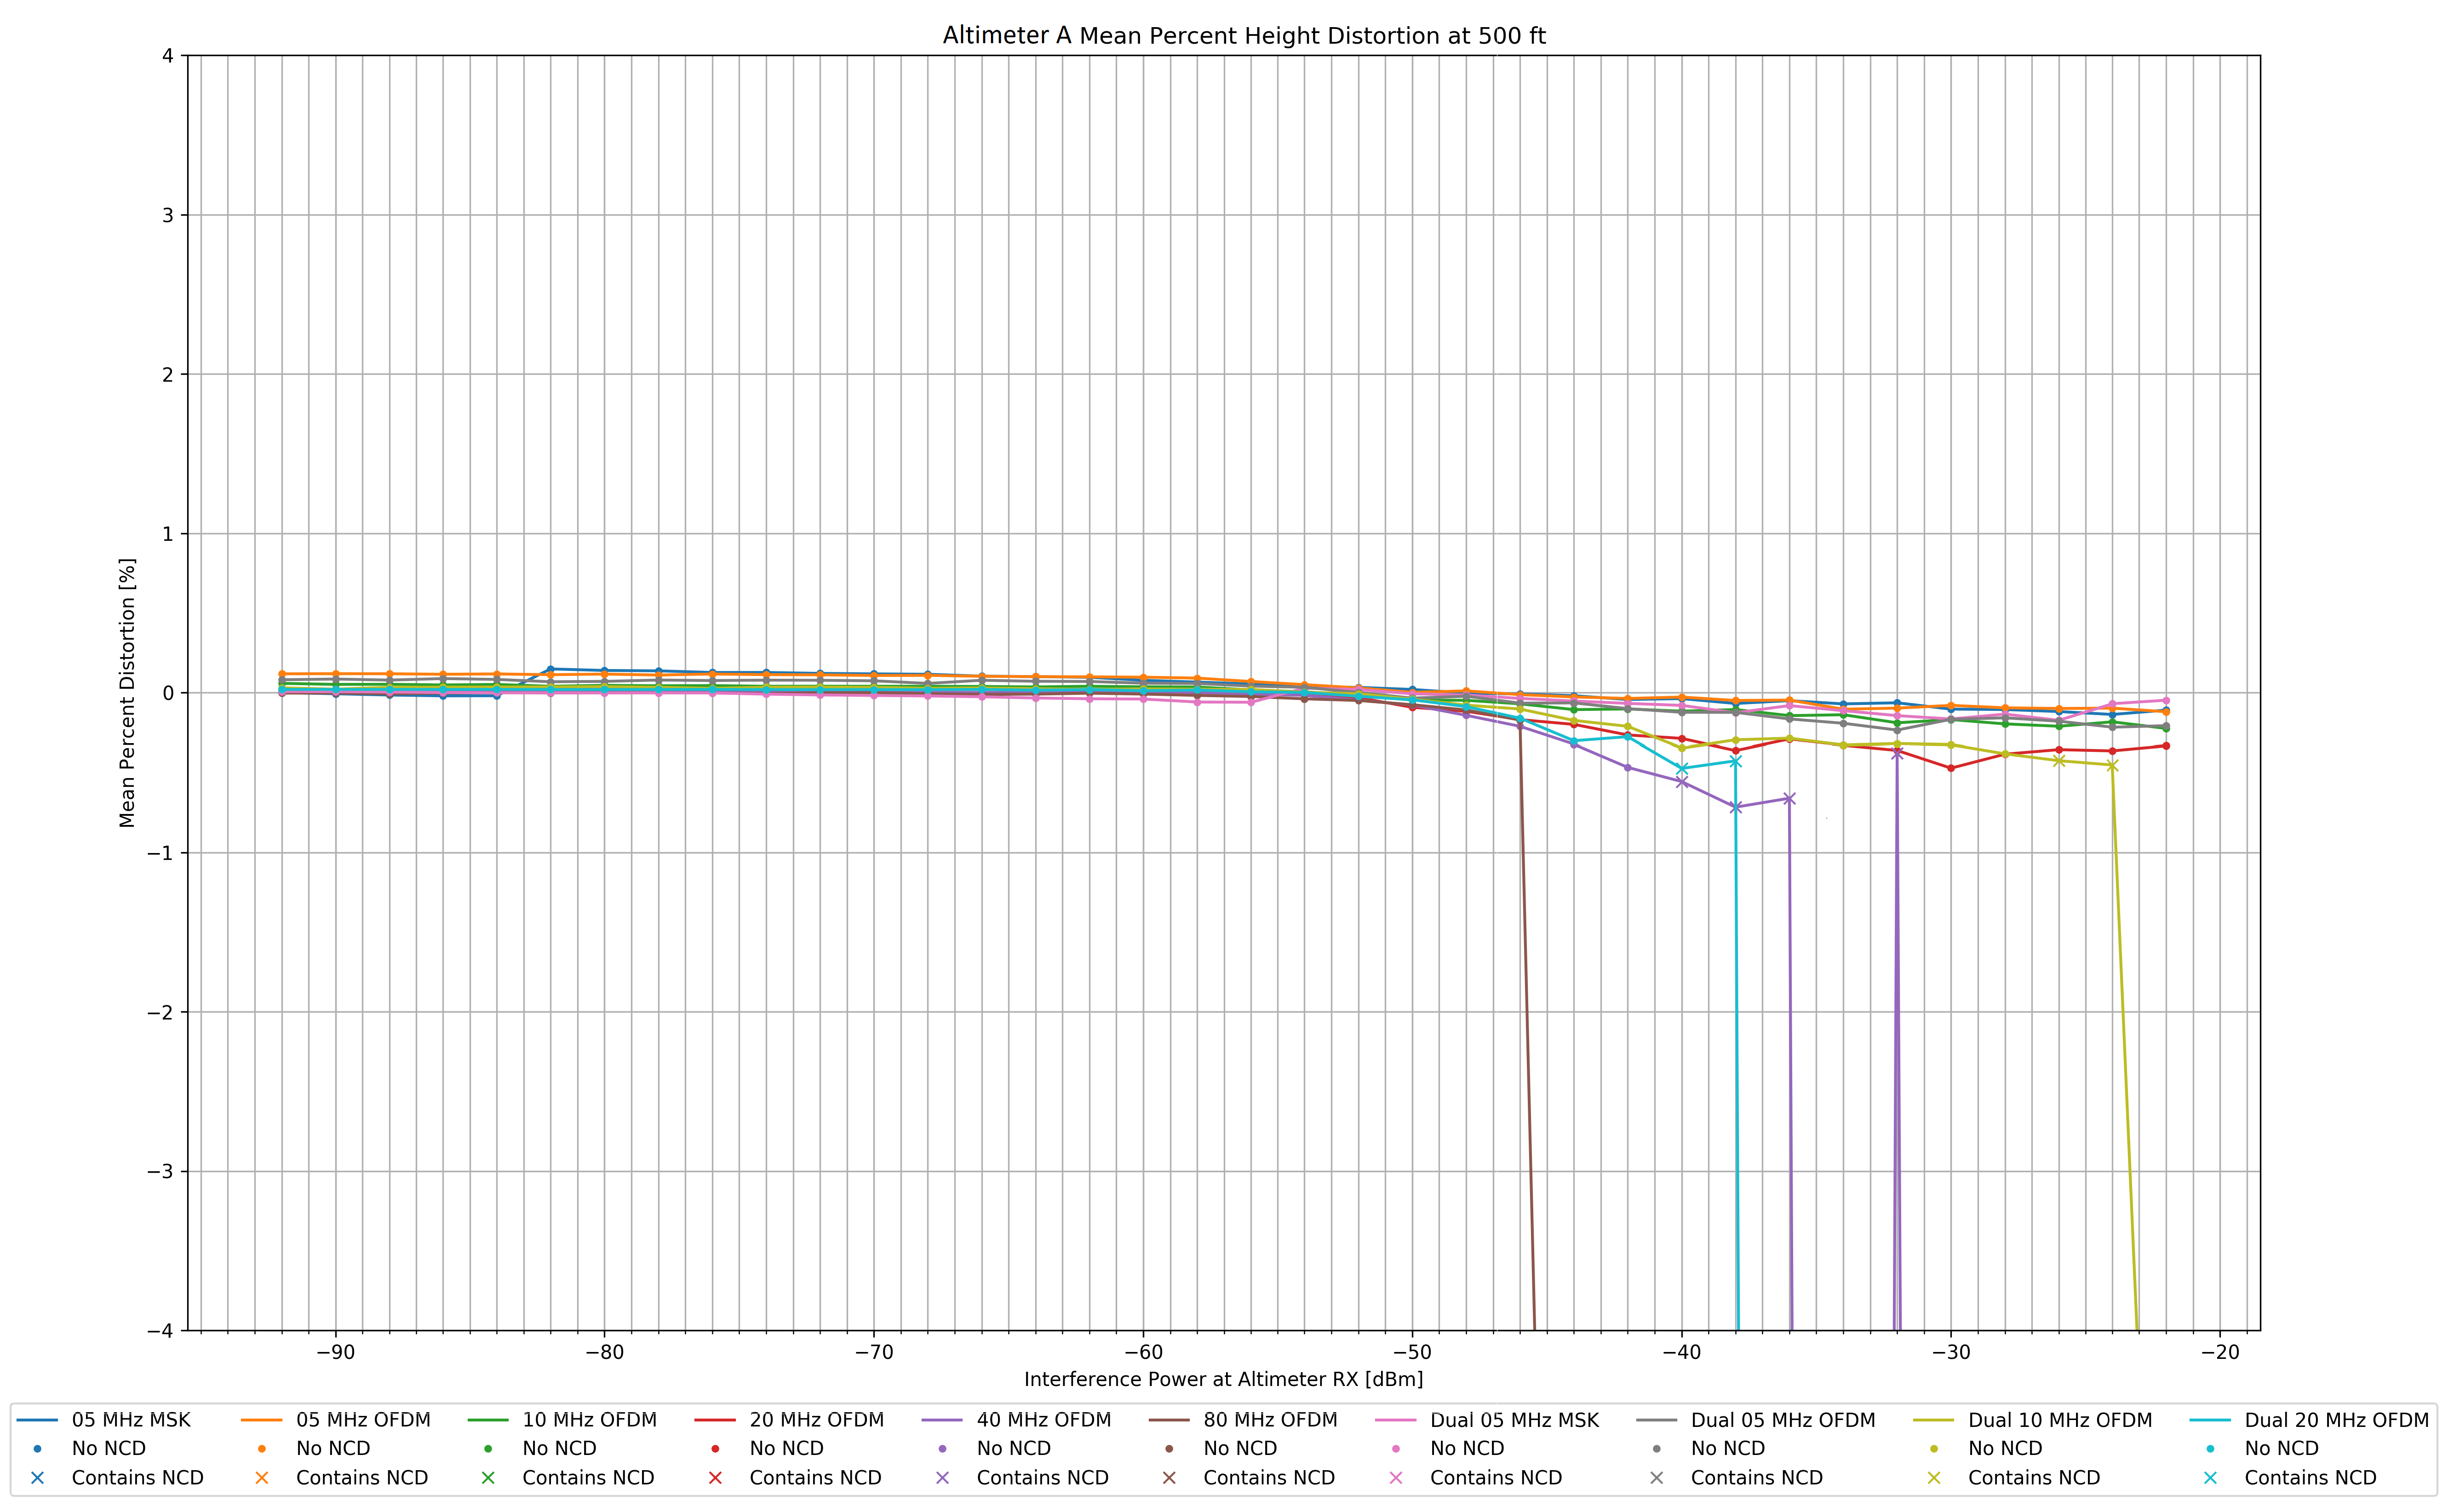
\includegraphics[width=6.0in]{Mean_Comparison_Example.png}
	\caption{Comparison of Impact of Different Bandwidths of Simulated WAIC Signals on Altimeter Performance}
	\label{fig:mean_comparison}
\end{figure}
Finally, these tests investigated the effects of interference bandwidth on altimeter performance, and the effects of separating a waveform into a `dual' version of the waveform with a $\pm20$ MHz offset from the center. The test definition shown in Table~\ref{tab:initial_signals} was the last iteration of the test procedure run before expanding the setup, and functions to demonstrate these effects. Figure~\ref{fig:mean_comparison} shows a stat plot comparing the mean height error caused by interference signals of increasing bandwidth. These results consistently showed that wider bandwidth interference caused worse altimeter performance. Although dual waveforms helped performance, their impact was inconsistent.  

These results were used to justify expanding the test setup and measuring altimeter response to wider bandwidth WAIC signals aggregated with interference from other altimeters to provide a realistic worst case scenario.

\section{Expanded In Band Tests}\label{sec:dvsg_ib_results}
This section discusses the results of the testing regimen described in Section~\ref{sub:ib}. The goal of this iteration of tests was to measure the response of altimeters to a full band of simulated WAIC interference, in the presence of simulated interference from other altimeters. The combined interference represented a more conservative than the real life worse case scenario for altimeter interference. 5 different altimeters were tested: the Rockwell Collins LRA2100, The Rockwell Collins LRA900, the Thales ERT530, the Thales ERT550, and the Honeywell ALA52B.
 \begin{figure}[h!]
	\centering
	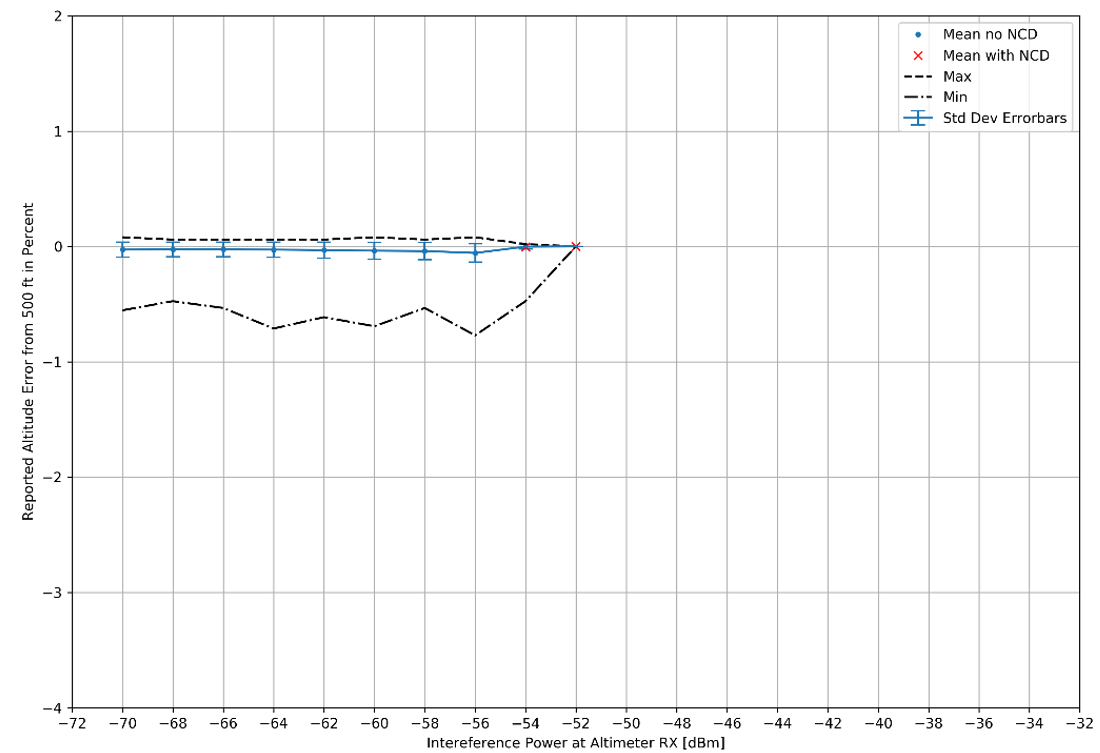
\includegraphics[width=6.0in]{RA4_ib_results.png}
	\caption{Performance of RA Type 4 with 200MHz In Band Tests}
	\label{fig:RA4}
\end{figure}

 % Please add the following required packages to your document preamble:
% \usepackage{booktabs}
\begin{table}[]
\begin{tabular}{@{}cccccc@{}}
\toprule
                            & RA Type 1 & RA Type 2 & RA Type 3 & RA Type 4 & RA Type 5 \\ \midrule
WAIC Interference Threshold & -54 dBm   & -56 dBm   & -44 dBm   & -56 dBm*  & -44 dBm   \\ \bottomrule
\end{tabular}
\caption{Interference power level above which reported altitude is impacted~\cite{uwe_radio_2019}}
\label{tab:ib_thresholds_fsmp}
\end{table}

 The breaking point of each was found according to Section~\ref{sub:break}, and these were used to propose maximum radiated power thresholds to the FSMP~\cite{uwe_radio_2019}. The resulting minimum power thresholds, with altimeter names redacted, are shown in Table~\ref{tab:ib_thresholds_fsmp}. RA Type 4 performed the worst of the 5 models tested, so the final threshold recommended to the FSMP was 56 dBm based on this failure point. Figure~\ref{fig:RA4} 
 shows the results of this altimeter. The first breaking point occurs at -54 dBm interference power at the altimeter receiver, thus the WAIC threshold was set at -56 dBm. The results of the remaining altimeters are shown in Appendix~\ref{appendix_a} for completeness. 

\section{Out of Band Testing}\label{sec:dvsg_oob_results}
 \begin{figure}[h!]
	\centering
	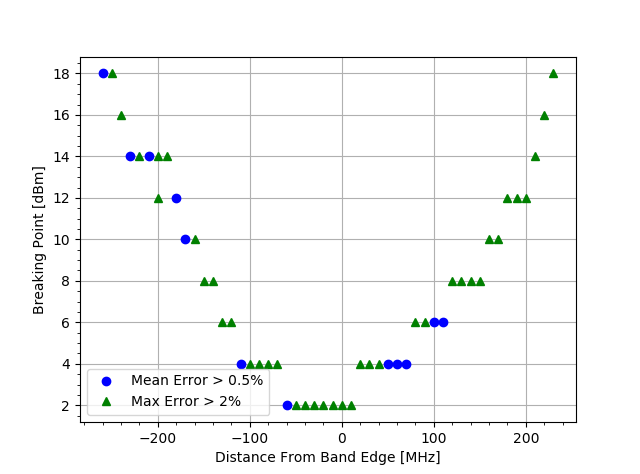
\includegraphics[width=3.5in]{oob_mask.png}
	\caption{Preliminary Interference Mask}
	\label{fig:oob_mask}
\end{figure}

This section covers the results of the out of band testing regimen described in Section~\ref{sub:oob}. This test used the same expanded test setup as the 200 MHz in band tests. VCOs were used to simulate external altimeter signals at a 200ft approach, and one of the VSG's generated 130 MHz wide simulated WAIC interference. The second VSG stepped RF signals out from the band edges. The goal was to find how the breaking point changed with distance from the band edge in MHz. An example of these results plotted is shown in Figure~\ref{fig:oob_mask}. These tests are still in progress at the time of writing, but like the results in Section~\ref{sec:dvsg_ib_results}, are expected to justify reccomendations made to regulators for safe power thresholds in the adjacent bands. 

